The game being challenging confines largely to item 2, but also items 5 and 6 from the requirements in section \ref{gamedesign:selectionofgametype:importantstuff}.
The challenge in the game is the horde of enemies that chase the player, but if the enemies are all stuck behind a wall the challenge is non-existent.
Therefore the enemies need to be able to avoid obstacles and chase the players in a intelligent way.
This could be achieved by applying a pathfinding algorithm to the AI's behaviour.

\section{Pathfinding}
%Gridbased graph: 3984 nodes, 30450 edges
%Waypoint graph: 47 nodes, 624 edges

The pathfinding algorithm that we will be using is A* search pathfinding which has a runtime of $O(n*m)$, where n is the number of nodes that will be explored, m is the average number of neighbours in the graph, and we assume that the graph and heuristic operations take constant time \cite{AIG:Millington}.
%Other pathfinding possibilities would be BFS or floyd-warshall algorithm, but as BFS has a runtime of [] and floyd-warshall has a runtime of [] with a high memory usage, we will not be using them.

The first step in using an A* search algorithm, is to have a proper graph which represents the map in the game.
Our initial idea was to simply have each walkable square in the grid to be a node.
A node would then have up to eight connections which would point to a neighbour of that certain node with a cost of traversing to this node.
Possible neighbours would be four to each side of the node with a cost of 10 and four diagonal neighbours with a cost of 14, which is the length of the hypotenuse when the length of the catheti are 10.
This approach resulted in a very large graph which took a lot of time to create and traverse through, when running the algorithm on it.
An example of this can be seen in figure \ref{gridGraph} where you can see a map of size 64x64, the graph created for that map has 3984 nodes and 30450 edges.

\begin{figure}[H]
	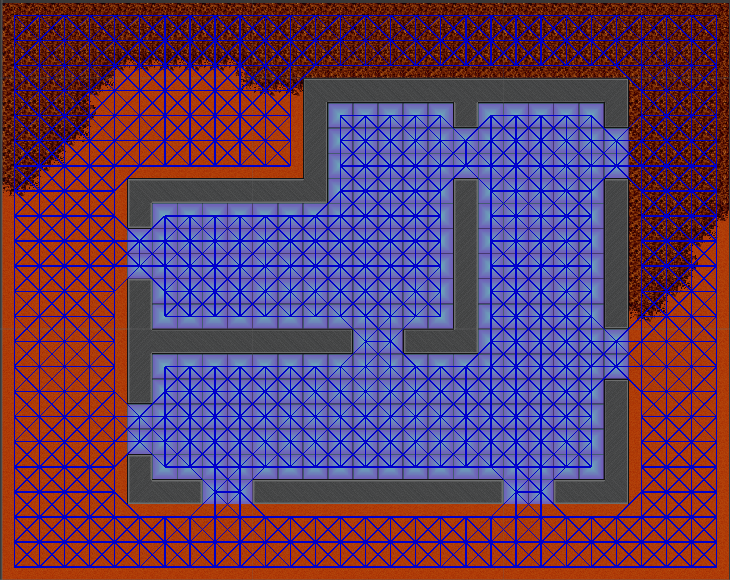
\includegraphics[width=\textwidth]{figures/astar/gridGraph}
	\caption{Graph based on the grid of the map}
	\label{gridGraph}
\end{figure}

An optimisation for to this was to change the graph from being grid based to a waypoint graph.
We would create the graph based on the outer corners of the obstacles on the map, where the AI had to make a turn, as seen in figure \ref{waypointsNode}.
Each point would then do a check on every other point to see if it was in direct sight, if that was the case it was added as a neighbour and the cost for that edge would be the euclidean distance to that point.
A resulting graph can be seen in figure \ref{waypointgraph}.
This approach resulted in a much smaller graph with 47 nodes and 624 edges, thus improving both the creation of the graph and the traversal of it.

\begin{figure}[H]
	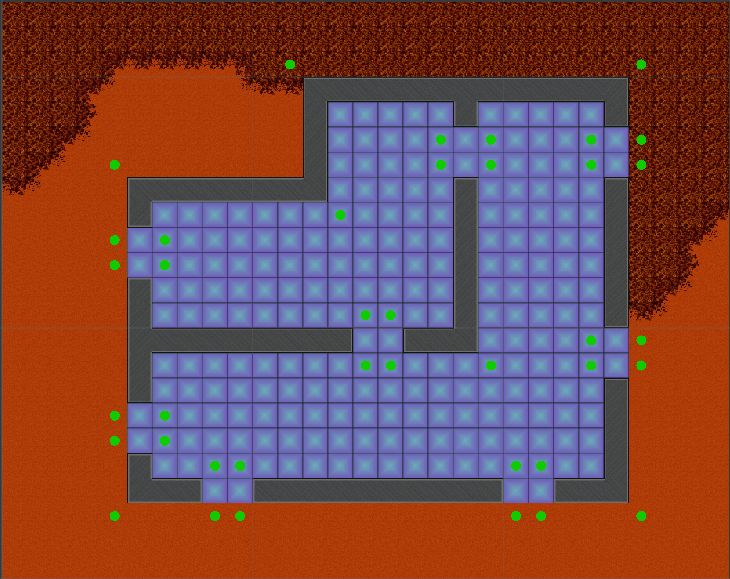
\includegraphics[width=\textwidth]{figures/astar/waypoints}
	\caption{The placement of the waypoints}
	\label{waypointsNode}
\end{figure}

\begin{figure}[H]
	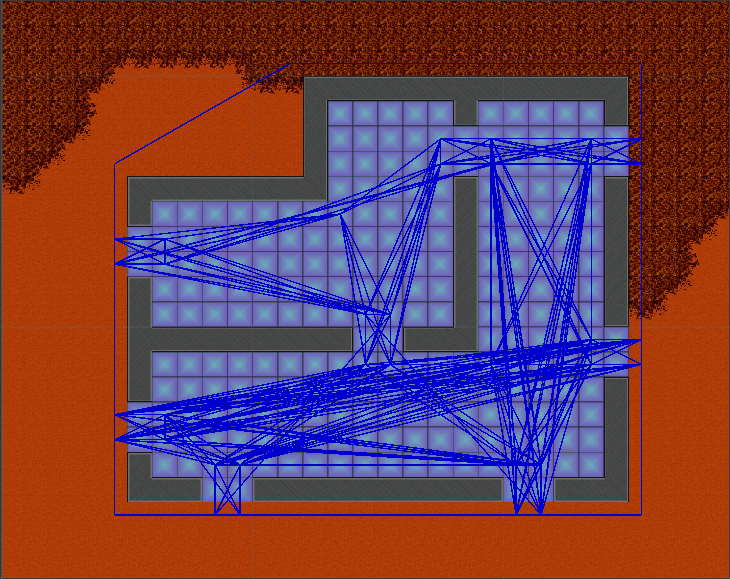
\includegraphics[width=\textwidth]{figures/astar/waypointsGraph}
	\caption{Graph based on the waypoints}
	\label{waypointgraph}
\end{figure}

Running an A* search pathfinding from every enemy is computationally costly which lead us to futher optimise pathfinding.
First optimisation is to check whether the player is in direct line of sight in which case we can go straight towards the player and not execute any pathfinding algorithm.
If the player then runs out of sight, we can still continue to walk towards the position where the player was last seen and once we have reached that position we look for the player again.
When the player is not in sight, we check for surrounding enemies who perhaps have run the pathfinding algorithm and are on their way towards the player, then we simply follow this entity.
When neither of the above options are available, we run the pathfinding algorithm and follow the path until we have the player in sight again or reached the end of the path where we then have to run the algorithm again.

\begin{figure}[H]
	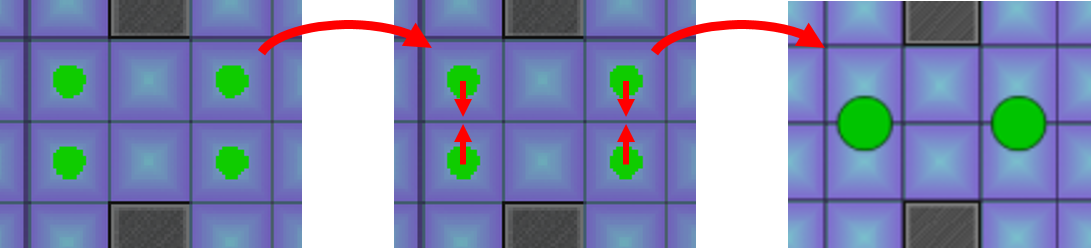
\includegraphics[width=\textwidth]{figures/astar/waypointMerge}
	\caption{Waypoint merging.}
	\label{waypointMerge}
\end{figure}

This is still an expensive algorithm, so in order to optimize further, an effor is made to reduce the number of redundant waypoints.
All waypoints are looped through to find adjacent waypoints, meaning waypoints whose distance to each other is less or equal to one.
Those that are adjacent are then removed and a new waypoint is placed halfway between them.
This is illustrated in Figure \ref{waypointMerge}.
The resulting waypoints can be seen in Figure \ref{waypointOpt} with the graph in Figure \ref{waypointgraphOpt}.
Most notably, the amount of edges are significantly reduced.

\begin{figure}[H]
	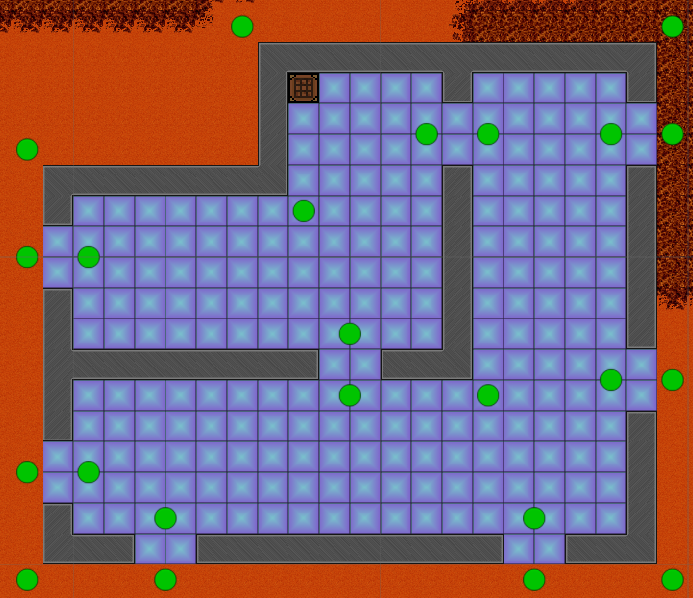
\includegraphics[width=\textwidth]{figures/astar/optimizedWaypoints}
	\caption{Waypoints after optimizations.}
	\label{waypointOpt}
\end{figure}

\begin{figure}[H]
	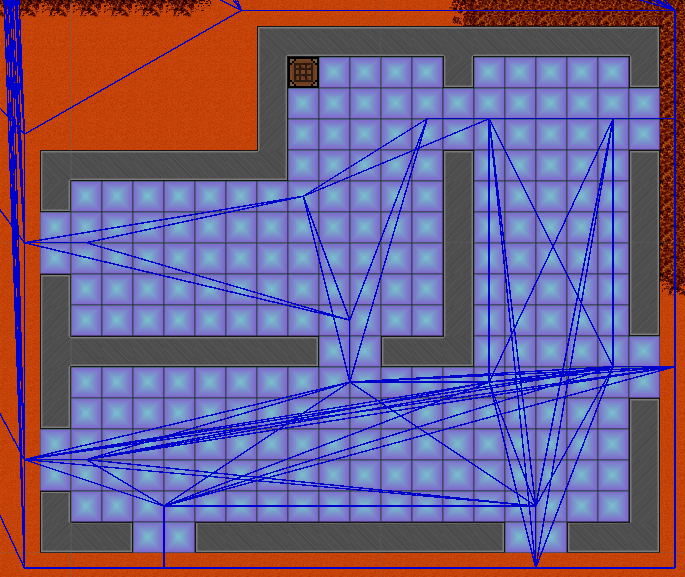
\includegraphics[width=\textwidth]{figures/astar/optimizedWaypointsGraph}
	\caption{Graph based on the waypoints after waypoint optimization.}
	\label{waypointgraphOpt}
\end{figure}


